\chapter{Validation}

\par The experiment was carried out over the first half of the Spring 2017 quarter at Cal Poly. 130 students signed up across 4 classes. By the end of the experiment, just over 3200 answers had been submitted to the application.

\section{Data Gathering}

\subsection{Midterm Scores}
\par In order to gauge the effectiveness of \textit{Polycommit}, we collected scores on quizzes and exams and aggregated the data to be analyzed. For \textbf{Introduction to Operating Systems}, data collection was extremely simple as all the quizzes and midterms were administered through an online exam. This allowed us to easily obtain data on how students performed on specific midterm questions that aligned with questions asked in \textit{Polycommit}.

\par However, the other classes were not as simple. The other classes administered paper midterms, and we did not have access to the papers as they were being graded. As such, we administered a secondary survey to all the students in the class asking them to input their midterm scores for various questions.

\subsection{Final Survey}
\par After the experiment was concluded, all participants were sent a link to a survey where they could give feedback about their overall experience using \textit{Polycommit}. As an incentive, any participant who filled out the survey received +3 Commitment and +50 points (equal to an additional entry in the gift card raffle). A total of 70 participants filled out the post-experiment survey.

\subsection{Limitations}
\par Certain tradeoffs were necessary in order to run this experiment.
\subsubsection{No Control Group} 
\par Most importantly, there is no true control group for this experiment. We decided that it would be more advantageous to offer the application to all students in each section of the classes. This simplified the onboarding process, as we could present the application to all members of the class at once, and allow anyone to sign up. It also prevented potential issues where students might perceive it as unfair that certain students were give access to a study resource and others were not. In addition, this allowed more students to participate in the experiment, giving us access to more data and more user feedback.

\par As such, it's important to note that the students who participated in the study \textbf{self-selected} to become part of the experiment. Students who \textbf{did not} use the app can't be considered a control group, because they are not a random selection from the whole population. Allowing students to self-select may have introduced confounding variables. For example, perhaps students who are confident in their study techniques would choose to not participate, making the average midterm scores higher for non-participants.

\subsubsection{Self-Reporting Midterm Scores}
\par As noted above, students were asked to input their midterm scores in an online form. We have no way of determining if this data was accurately entered; students may feel tempted to enter a higher score than they actually received. Note that we \textit{do} have access to the overall midterm scores, so the issue only arises when analyzing individual questions on the exams. Data that has been affected by this issue is clearly marked in the upcoming sections.

\section{Overall Results}
\subsection{Cramming vs. Commitment}
\par First, consider the relationship between a student's overall score on the midterm and their Commitment (\textbf{\hyperref[fig:comm_vs_score]{Figure \ref*{fig:comm_vs_score}}}). 
 
 \begin{figure}[ht]
 	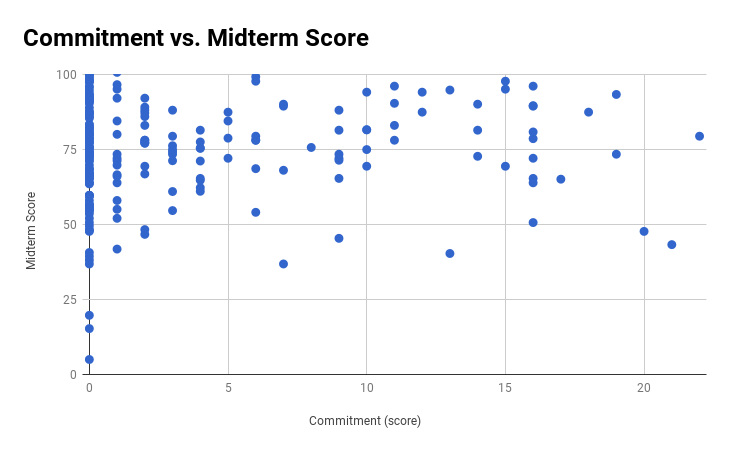
\includegraphics[width=1.0\linewidth]{figures/commitment-data1}
 	\caption{Graph of Commitment versus the student's percentage score for all classes.}
 	\label{fig:comm_vs_score}
 \end{figure}

\par Note that we are showing the midterm percentage score, since the midterms in different classes have different total score values.
\par There is no clear correlation between a user's Commitment value and the score they got on the midterm. Thus, this data does not support the hypothesis that using spaced repetition to study for an exam improves the user's score.

\par  Next, we can compare the total number of questions answered by each user with their midterm score (\textbf{\hyperref[fig:cramming]{Figure \ref*{fig:cramming}}}). If students received a benefit from the Commitment system, we might expect to see \textit{less} of a correlation between total questions answered and midterm score. This is because if a user has a high number of questions answered but a low Commitment, this indicates they answered the questions all at once, in a "cram" session. According to our hypothesis, this would not help improve their long-term understanding of the course.

\begin{figure}[ht]
	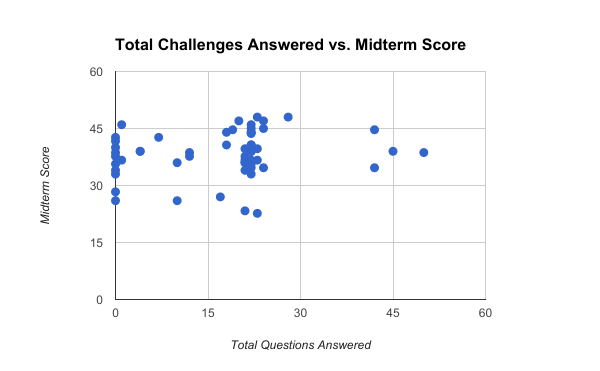
\includegraphics[width=1.0\linewidth]{figures/cramming-data}
	\caption{Graph of Total Questions Answered vs. the student's score on the midterm.}
	\label{fig:cramming}
\end{figure}
 
 \par Next, consider the mean of all midterm scores between students that didn't answer \textit{any} questions vs. the ones that did. For all classes except CPE 471, students that didn't answer any questions in the app scored slightly higher on average than the students that didn't. The discrepancy in CPE 471 is most likely due to the smaller number of students that signed up for \textit{Polycommit}.
 
 \par Note that we define "Active Users" as any user with over 5 Commitment. 
  
  \begin{table}
 \begin{tabular}[h]{ r c c c}
  & \textbf{Non-users} & \textbf{All Users} & \textbf{Active Users} \\
  \hline
  \textbf{All Classes} & & & \\
  Midterm Average & 72.93 & 76.12 & 76.88 \\
  Population Size & 119 & 103 & 87 \\
  \hline
  \textbf{CPE 453} & & & \\
 Midterm Average & 74.38 & 77.56 & 77.40 \\
 Population Size & 14 & 46 & 42 \\
 \hline
 \textbf{CPE 464} & & & \\
 Midterm Average & 68.90 & 73.85 & 76.08 \\
 Population Size & 47 & 42 & 34 \\
 \hline
 \textbf{CPE 471} & & & \\
 Midterm Average & 87.38 & 82.39 & 83.83 \\
 Population Size & 34 & 7 & 4 \\
 \hline
 \textbf{MATH 244} & & & \\
 Midterm Average & 74.43 & 85.87 & 85.87 \\
 Population Size & 26 & 11 & 10 \\
 
\end{tabular}
\caption{Average midterm scores for different samples of the population. Note that an "Active User" is a user with more than 5 Commitment.}
\end{table}

\subsection{Individual Questions}
Certain questions on the midterm matched closely with the content of the questions that were repeated on \textit{Polycommit}. We can analyze midterm results to see if the students that drilled related problems in \textit{Polycommit} performed better on the related questions during the midterm.

\subsubsection{Introduction to Operating Systems}
One question that was shared between the midterm and \textit{Polycommit} was a question about the 4 conditions for deadlock. The question on the midterm asked students to choose the correct 4 conditions from a series of dropdowns, while the question on \textit{Polycommit} asked students to choose the \textit{incorrect} condition from the list. The 4 conditions for deadlock are:

\begin{enumerate}
	\item \textbf{Mutual exclusion}: At least one resource can only be
	held by one process at a time; this can result in other
	processes waiting for that resources
	\item \textbf{Hold and wait}: A process must be holding at least one
	resource while waiting for other resources (held by other
	processes)
	\item \textbf{No preemption}: Resources can only be released
	voluntarily by a process; Resources cannot be revoked
	\item \textbf{Circular wait}: A set of n waiting process $ {P_0, ..., P_n} $
	such that $ P_i $ is waiting for resources held by $ P_{(i+1)\%n} $
\end{enumerate}

\par The content of the question in \textit{Polycommit} and the question in the midterm are very similar. We can see if individuals who answered the Deadlock question correctly in \textit{Polycommit} had a higher score, on average, than the individuals who did not.

\begin{figure}[th!]
	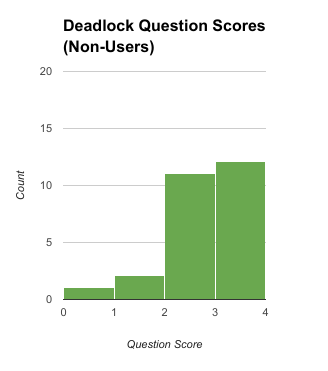
\includegraphics[width=0.5\linewidth]{figures/deadlock-nonusers}
	\caption{Count of scores for students that did \textit{not} make an attempt on the Deadlock question in \textit{Polycommit}.}
	\label{fig:deadlock-no}
\end{figure}

\begin{figure}[h!b]
	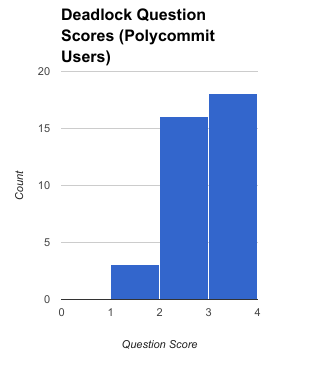
\includegraphics[width=0.5\linewidth]{figures/deadlock-users}
	\caption{Count of scores for students that \textit{did} make an attempt on the Deadlock question in \textit{Polycommit}.}
	\label{fig:deadlock-yes}
\end{figure}

\par The mean score for \textbf{non-users} is 3.30, and the mean score for \textbf{users} is 3.31. Thus, using \textit{Polycommit} had a negligible effect on the average score of the participants. However, note that 23/26 \textbf{non-users} received a score greater than 3, while 34/37 \textbf{users} received a score greater than 3. This could reflect the fact that \textit{Polycommit} only referenced 3 out of the 4 conditions for deadlock, as the 4th condition in the problem was a false plant. Although all 4 conditions are listed in the "explanation" field for the problem, by default if a student answers the question correctly they are brought back to the course page. Thus, students who participated in \textit{Polycommit} were only drilled on 3 out of the 4 conditions for deadlock, which would explain the overall performance on the midterm.

\par Next, we will examine problems related to scheduling. Scheduling, in Operating Systems, is the process by which a multithreaded CPU decides which processes get to run at a certain time. Since scheduling problems are easy to generate and automatically grade, several such problems were included in \textit{Polycommit}. Below, we graph the amount of scheduling problems users answered in \textit{Polycommit} versus the score they got on the scheduling section of the midterm.

% TODO: also include graph where people got the polycommit question incorrect

\begin{figure}[h!b]
	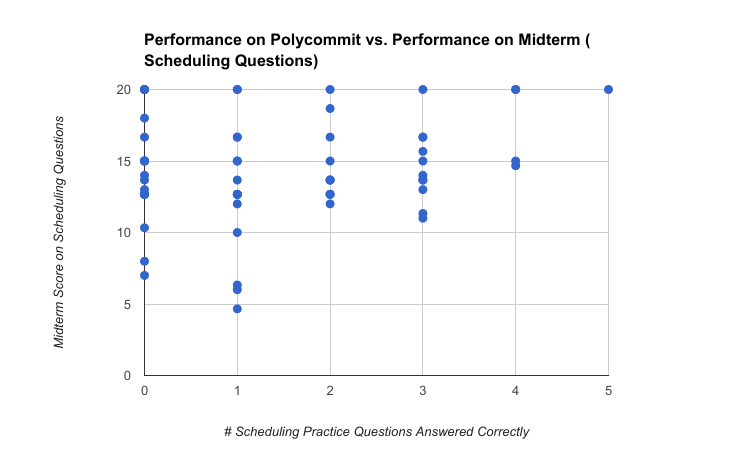
\includegraphics[width=1.0\linewidth]{figures/scheduling}
	\caption{Scatter plot where the X axis is the amount of scheduling problems the user answered on \textit{Polycommit}, and the Y axis is the total score they received on the 4 scheduling questions of the midterm.}
	\label{fig:scheduling}
\end{figure}

\par As you can see, there is a clear correlation between consistently practicing scheduling questions and performing well on the exam. While many students did get full credit on the scheduling portion of the exam, the students who answered all 5 scheduling questions on Polycommit all scored perfectly on that section of the exam.

%TODO do the "see figure x" thing

\subsubsection{Introduction to Computer Graphics}

\par Questions about \textbf{vector math}, \textbf{transformation matrices}, and \textbf{barycentric coordinates} were practiced in \textit{Polycommit}, and were subsequently tested on the midterm for Computer Graphics. Below is a table displaying the midterm performance of students who answered questions about each question on \textit{Polycommit}.

\begin{table}
	\begin{tabular}[h!]{ r c c }
		& \textbf{Did practice} & \textbf{Did not practice} \\
		\hline
		\textbf{Vector Math} & & \\
		Score & 98\% & 100\%  \\
		
		\hline
		\textbf{Transformation Matrices} & &  \\
		Score  & 92.1\% & 86.3\% \\
		
		\hline
		\textbf{Barycentric Coordinates} & &  \\
		Score  & 100\% & 97.7\% \\
		
		\caption{IMPORTANT: These midterm scores were self-reported, so their accuracy depends on the honesty of the reporting student.}
	\end{tabular}
\end{table}

\subsubsection{Introduction to Computer Networks}

\par Questions about \textbf{IP Addressing}, \textbf{CRC Checksums} and \textbf{sliding window protocol} were practiced in \textit{Polycommit}, and were subsequently tested on the midterm for Computer Networks. Below is a table displaying the midterm performance of students who answered questions about each question on \textit{Polycommit}.

\begin{table}
	\begin{tabular}[h!]{ r c c }
		& \textbf{Did practice} & \textbf{Did not practice} \\
		\hline
		\textbf{IP Addressing} & & \\
		Score & 80\% & 77.4\%  \\
		
		\hline
		\textbf{CRC Checksums} & &  \\
		Score  & 100\% & 86.3\% \\
		
		\hline
		\textbf{Sliding Window Protcol} & &  \\
		Score  & 90\% & 76.9\% \\
		
		\caption{IMPORTANT: These midterm scores were self-reported, so their accuracy depends on the honesty of the reporting student.}
	\end{tabular}
\end{table}

\section {User Feedback}

\par At the end of the experiment, we contacted all of the participants with a final survey that asked them questions about their usage of the app. It also included two free-response questions that asked users to offer suggestions about how the app could be improved.

\subsection{Rating Summary}

\par The full survey is viewable in \textbf{\hyperref[fig:survey1]{Figure \ref*{fig:survey1}}}. Users responded to several statements about the app using a standard Likert scale ranging from Strongly Disagree to Strongly Agree. A summary of the user responses is available at \textbf{\hyperref[fig:likert]{Figure \ref*{fig:likert}}}. Notably, a majority of users responded quite positively to the app.


\begin{figure}[h]
	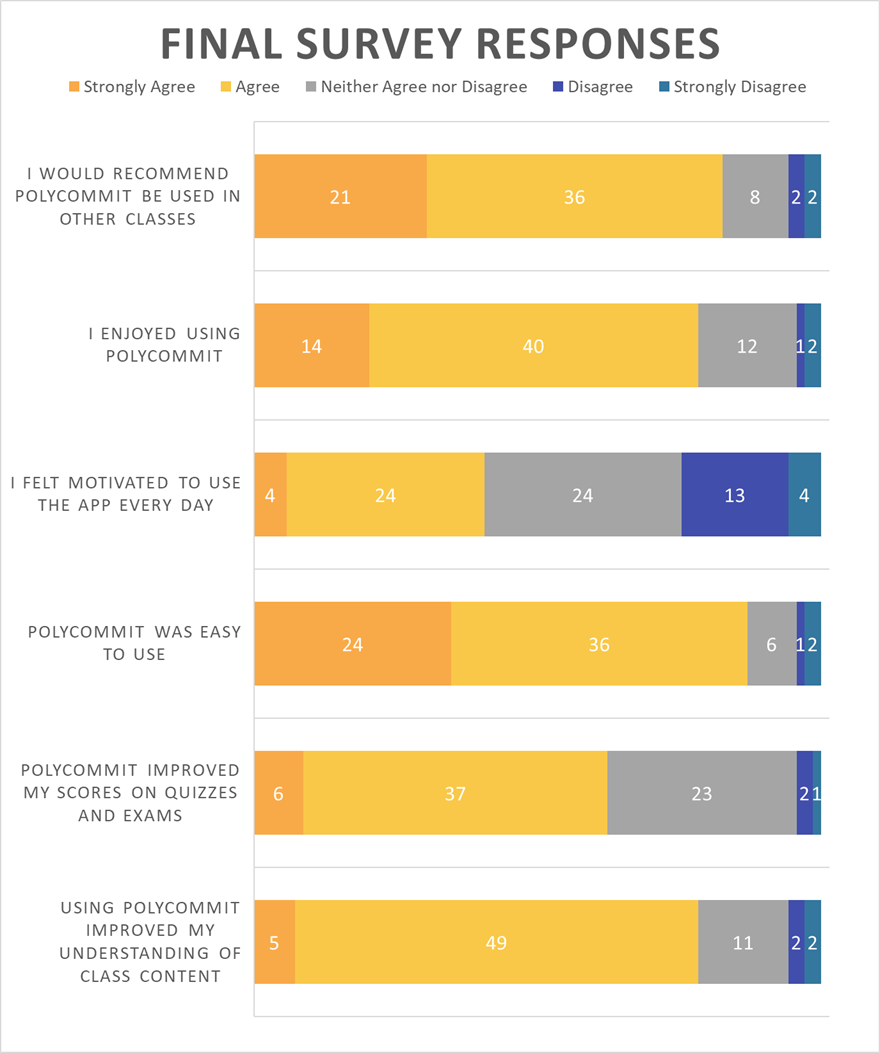
\includegraphics[width=1.0\linewidth]{figures/likert}
	\caption{Survey responses from users of Polycommit.}
	\label{fig:likert}
\end{figure}

\subsection{User Self-Evaluation vs. Actual Scores}

\par One interesting result comes by grouping midterm scores by the user's response to "\textit{Polycommit} improved my scores on quizzes and exams" (See \textbf{\hyperref[fig:overconfidence]{Figure \ref*{fig:overconfidence}}}). Students who reported that \textit{Polycommit} did \textit{not} improve their scores scored substantially higher than students who did. One explanation for this is that students who were already confident about their studying habits or had prior knowledge of Operating Systems did not feel that \textit{Polycommit} had an impact on their grades, which are already high overall.

\begin{figure}[h]
	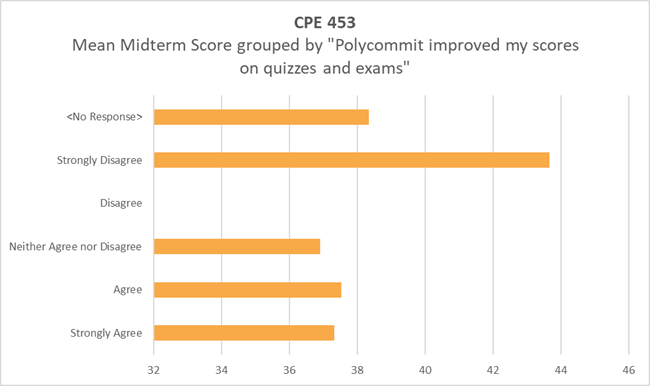
\includegraphics[width=1.0\linewidth]{figures/improved-vs-score}
	\caption{Mean midterm score grouped by response to final survey question "\textit{Polycommit} improved my scores on quizzes and exams."}
	\label{fig:overconfidence}
\end{figure}


\subsection{Free Response Summary}
\par Before viewing the results, we predicted some categories that user responses might fall into. These categories are:

\begin{enumerate}
	\item Problems or confusions with the user interface
	\item Questions were not correct or were confusing
	\item Questions did not represent test material
	\item App needed more gamification, excitement, or incentive to use
	\item Other
\end{enumerate}

\par The total number of responses that fell under each category are:

\vspace{1.0cm}

\begin{tabular}{ r c }
	\textbf{Category} & \textbf{\# Responses} \\
	Problems or confusions with the user interface & 26 \\
	Questions were not correct or were confusing  & 9 \\
	Questions did not represent test material  & 5 \\
	App needed more gamification, excitement, or incentive to use  & 1 \\
	Other  & 29 \\
\end{tabular}

\vspace{2.0cm}

\par The full list of responses is available below. Note that answers \textit{are} shown when a question is closed, so feedback asking for answers to be displayed is filed under "UI Issues" since the problem is essentially that the app failed to present the information in a way that users could find it.


% Please add the following required packages to your document preamble:
% \usepackage[normalem]{ulem}
% \useunder{\uline}{\ul}{}
\renewcommand*{\arraystretch}{2.0}
{\fontsize{12pt}{8pt}\selectfont
\newcolumntype{R}{>{\raggedleft\arraybackslash}p{0.2\linewidth}}
\begin{longtable}{R|p{0.8\linewidth}}
	
	\label{feedback-table}
	\textbf{CATEGORY} & \textbf{RESPONSES} \\
	\hline
		\textbf{User Interface Problems} &  - There are some UI problems that could be fixed. Certain values like points and commitment weren't consistent from page to page.\newline-   Solving the can't see answers even if actually trying was kind of frustrating\newline-   I think this might be more useful if there was an app version with a notification each day. I wanted to keep up with Polycommit, but it's pretty easy to forget to check in from day to day. \newline-   Polycommit had one question a day, but the study guide had 70 questions on it. As a result, it wasn't as helpful as I expected it to be because by the time of the exam, I feel like a large portion of the class material didn't show up as a question on polycommit. \newline - Ability to review questions would be nice \newline- Also, explanations for answers would be helpful                                                                                                                                                                                                                                                                                                                                                                                                                                                                                                                                                                                                          
		\newline - Ability to review the answers to questions                                                                                                                                                                                                                                                                                                                                                                                                                                                                                                                                                                                                                                                                                                       \\
		 & After missing all the allowed attempts, it would be nice to know what the answer is so we have a solution to work backwards from. Overall, however, the site was clean and easy to use.                                                                                                                                                                                                                                                                                                                                                                                                                                                                                                                                                          \\
		& Explanation if you keep missing the answer to the question.                                                                                                                                                                                                                                                                                                                                                                                                                                                                                                                                                                                                                                                                                      \\
		& Feedback box, more closely tie in with a professor's class                                                                                                                                                                                                                                                                                                                                                                                                                                                                                                                                                                                                                                                                                       \\
		& fix all the bugs                                                                                                                                                                                                                                                                                                                                                                                                                                                                                                                                                                                                                                                                                                                                 \\
		& Give us answers!                                                                                                                                                                                                                                                                                                                                                                                                                                                                                                                                                                                                                                                                                                                                 \\
		& I realized that to earn unique commitment days it runs off of a 24 hour period and not actual days on a calendar. Maybe put a timer?                                                                                                                                                                                                                                                                                                                                                                                                                                                                                                                                                                                                             \\
		& Including the correct answer so you aren't left wondering                                                                                                                                                                                                                                                                                                                                                                                                                                                                                                                                                                                                                                                                                        \\
		& It would be nice to be given the correct answer if I answer incorrectly too many times. Also, the worked out solution would be helpful.                                                                                                                                                                                                                                                                                                                                                                                                                                                                                                                                                                                                          \\
		& Make previous questions easily accessible like having an answered questions bank                                                                                                                                                                                                                                                                                                                                                                                                                                                                                                                                                                                                                                                                 \\
		& Mobile friendliness                                                                                                                                                                                                                                                                                                                                                                                                                                                                                                                                                                                                                                                                                                                              \\
		& Provide some sort of answer system. I understand that if you provide the answers then individuals can just use them to get answers; however, for people who are genuinely using your program, it was not very helpful if you go the answer wrong.                                                                                                                                                                                                                                                                                                                                                                                                                                                                                                \\
		& Providing an explanations for solutions after a student has missed it after a certain number of times could be beneficial.                                                                                                                                                                                                                                                                                                                                                                                                                                                                                                                                                                                                                       \\
		& Quick Feedback or flagging of questions that need to be reviewed. Also the UI could be improved a bit so it has better aesthetic appeal :)                                                                                                                                                                                                                                                                                                                                                                                                                                                                                                                                                                                                       \\
		& Remove the floating messages after a couple seconds, tell a user how many tries they have before they guess.                                                                                                                                                                                                                                                                                                                                                                                                                                                                                                                                                                                                                                     \\
		& Reporting the correct answer was sometimes confusing                                                                                                                                                                                                                                                                                                                                                                                                                                                                                                                                                                                                                                                                                             \\
		& See the answer if we didn't get it correct                                                                                                                                                                                                                                                                                                                                                                                                                                                                                                                                                                                                                                                                                                       \\
		& Show answers afterwards. Have a scheduled time a question will come out.                                                                                                                                                                                                                                                                                                                                                                                                                                                                                                                                                                                                                                                                         \\
		& Show the answer!                                                                                                                                                                                                                                                                                                                                                                                                                                                                                                                                                                                                                                                                                                                                 \\
		& Show the answers                                                                                                                                                                                                                                                                                                                                                                                                                                                                                                                                                                                                                                                                                                                                 \\
		& Showing answers after we run out of tries on a question, Having it be part of our grade (for incentive to use), having the teacher review the questions before putting them online                                                                                                                                                                                                                                                                                                                                                                                                                                                                                                                                                               \\
		& Some of the answers were not clear and did not show you how to do it, only gave you the correct answer. Showing the steps would be much appreciated! Other than that, very useful and helpful!                                                                                                                                                                                                                                                                                                                                                                                                                                                                                                                                                   \\
		& The software was a little buggy. The page often needed to be refreshed before displaying updated values.                                                                                                                                                                                                                                                                                                                                                                                                                                                                                                                                                                                                                                         \\
		& There were some minor issues with commitment points not being tracked on one page, but tracked on the other page.                                                                                                                                                                                                                                                                                                                                                                                                                                                                                                                                                                                                                                \\
		\hline
		\textbf{Incorrect or Confusing Questions} & Perhaps multiple choice would help a lot on questions whose answers can be more vagueAlso needs more memes                                                                                                                                                                                                                                                                                                                                                                                                                                                                                                                                                                                                                                       \\
		& Possibly offer more difficult questions as well. Maybe also add steps on how to arrive at the correct answer                                                                                                                                                                                                                                                                                                                                                                                                                                                                                                                                                                                                                                     \\
		& Some of the answer to the scheduling problems were wrong so it caused a lot of confusion.                                                                                                                                                                                                                                                                                                                                                                                                                                                                                                                                                                                                                                                        \\
		& Some of the answers for scheduling problems seemed to differ from the instructor's solution after the problem was shown to him.                                                                                                                                                                                                                                                                                                                                                                                                                                                                                                                                                                                                                  \\
		& some of the questions had answers that were too strict                                                                                                                                                                                                                                                                                                                                                                                                                                                                                                                                                                                                                                                                                           \\
		& Some of the questions have wrong answers and that could be checked.                                                                                                                                                                                                                                                                                                                                                                                                                                                                                                                                                                                                                                                                              \\
		& Sometimes the questions could be worded better                                                                                                                                                                                                                                                                                                                                                                                                                                                                                                                                                                                                                                                                                                   \\
		& There were some issues with correctness/clarity of questions. I also thought having worked out solutions for some of the more difficult problems would have been nice. Overall, I enjoyed using Polycommit. Thank you!                                                                                                                                                                                                                                                                                                                                                                                                                                                                                                                           \\
		& When the answers were incorrect or they didn't show the correct answer it really threw off my understanding of the material. I started to question a lot of what I thought I knew, and which ones of the questions were actually correct. This ended up really hurting me on the midterm, because I second guessed myself because of the PolyCommit questions that had been wrong that had not been fixed when I had last looked at them.                                                                                                                                                                                                                                                                                                        \\
		\hline
		\textbf{Questions Did Not Match Test} & Feedback box, more closely tie in with a professor's class                                                                                                                                                                                                                                                                                                                                                                                                                                                                                                                                                                                                                                                                                       \\
		& More relevant questions                                                                                                                                                                                                                                                                                                                                                                                                                                                                                                                                                                                                                                                                                                                          \\
		& Questions similar to what will be asked on tests and quizzes. Some sort of feedback when we get an answer correct. Maybe not the answer itself, but a hint or a point in the right direction of where to look for right answer                                                                                                                                                                                                                                                                                                                                                                                                                                                                                                                   \\
		& Some of the questions did not align correctly with the material we used in class and it would make more sense to have the weeks correspond to weeks in the quarter. I noticed that some of the questions continued to be posted in week 2 when were in week 4, etc.                                                                                                                                                                                                                                                                                                                                                                                                                                                                              \\
		& The app is great but the questions did not really follow the class material                                                                                                                                                                                                                                                                                                                                                                                                                                                                                                                                                                                                                                                                      \\
		\hline
		\textbf{Needed More Incentive} & More incentive to use it every day. I frequently forgot to do it everyday.                                                                                                                                                                                                                                                                                                                                                                                                                                                                                                                                                                                                                                                                       \\
		\hline
		\textbf{Other} & Add hints when a question is answered wrong.                                                                                                                                                                                                                                                                                                                                                                                                                                                                                                                                                                                                                                                                                                     \\
		& Adding an explanation for each solution would be very helpful.  Also more questions would be good.                                                                                                                                                                                                                                                                                                                                                                                                                                                                                                                                                                                                                                               \\
		& buzz notification to try a problem                                                                                                                                                                                                                                                                                                                                                                                                                                                                                                                                                                                                                                                                                                               \\
		& Emails or just a way to remind myself to do it every day!                                                                                                                                                                                                                                                                                                                                                                                                                                                                                                                                                                                                                                                                                        \\
		& Explain the answers in more depth                                                                                                                                                                                                                                                                                                                                                                                                                                                                                                                                                                                                                                                                                                                \\
		& Helpful links to textbook pages                                                                                                                                                                                                                                                                                                                                                                                                                                                                                                                                                                                                                                                                                                                  \\
		& I know people get a lot of emails in college, but maybe a reminder system could be created.                                                                                                                                                                                                                                                                                                                                                                                                                                                                                                                                                                                                                                                      \\
		& I think it would be nice to maybe have an optional daily reminder setting or some sort of notification system.                                                                                                                                                                                                                                                                                                                                                                                                                                                                                                                                                                                                                                   \\
		& I was never reminded to complete problems so I only did them the first week.                                                                                                                                                                                                                                                                                                                                                                                                                                                                                                                                                                                                                                                                     \\
		& I would love email notifications so that I remember to use it.                                                                                                                                                                                                                                                                                                                                                                                                                                                                                                                                                                                                                                                                                   \\
		& Instead of an answer, maybe add in a step by step solution                                                                                                                                                                                                                                                                                                                                                                                                                                                                                                                                                                                                                                                                                       \\
		& It would be nice to see the solutions to answers that you got wrong, where applicable.                                                                                                                                                                                                                                                                                                                                                                                                                                                                                                                                                                                                                                                           \\
		& Maybe I missed it, but I thought maybe this was an app? I could've been imagining things, but either way, I think that would be a great extension of the site! Also, I think a good addition might be reminders. Either phone notifications or emails. For those of us who are easily forgetful :)                                                                                                                                                                                                                                                                                                                                                                                                                                               \\
		& More clarity/ hints on difficult questions                                                                                                                                                                                                                                                                                                                                                                                                                                                                                                                                                                                                                                                                                                       \\
		& more questions                                                                                                                                                                                                                                                                                                                                                                                                                                                                                                                                                                                                                                                                                                                                   \\
		& More questions being posted                                                                                                                                                                                                                                                                                                                                                                                                                                                                                                                                                                                                                                                                                                                      \\
		& More questions per day would help. There's a lot of content to cover in CPE 464.                                                                                                                                                                                                                                                                                                                                                                                                                                                                                                                                                                                                                                                                 \\
		& More questions!                                                                                                                                                                                                                                                                                                                                                                                                                                                                                                                                                                                                                                                                                                                                  \\
		& More questions!  I know this was just a trial period, but more of the same would be greatly appreciated                                                                                                                                                                                                                                                                                                                                                                                                                                                                                                                                                                                                                                          \\
		& Notifications                                                                                                                                                                                                                                                                                                                                                                                                                                                                                                                                                                                                                                                                                                                                    \\
		& Perhaps some sort of remind feature for the daily question                                                                                                                                                                                                                                                                                                                                                                                                                                                                                                                                                                                                                                                                                       \\
		& Reminder emails                                                                                                                                                                                                                                                                                                                                                                                                                                                                                                                                                                                                                                                                                                                                  \\
		& Reminder emails or something like that could be really cool! There were some days when I just simply forgot to log on and do another question.                                                                                                                                                                                                                                                                                                                                                                                                                                                                                                                                                                                                   \\
		& Reminders via email (optional of course). Solution explanation/breakdown.                                                                                                                                                                                                                                                                                                                                                                                                                                                                                                                                                                                                                                                                        \\
		& Show the steps to the solution in order to better understand the material.                                                                                                                                                                                                                                                                                                                                                                                                                                                                                                                                                                                                                                                                       \\
		& Some notification service to remind you to complete it                                                                                                                                                                                                                                                                                                                                                                                                                                                                                                                                                                                                                                                                                           \\
		& The favicon reminds me of the ``browser tab crashed'' favicon.                                                                                                                                                                                                                                                                                                                                                                                                                                                                                                                                                                                                                                                                                     \\
		& The timing of the submission was odd. I would do it at a certain time and my commit would not increase                                                                                                                                                                                                                                                                                                                                                                                                                                                                                                                                                                                                                                           \\
		& Time Zone for updating score        
\end{longtable}
}



 